\documentclass[UTF8,a4paper,11pt]{ctexart}
\usepackage[left=22mm,right=22mm,top=23mm,bottom=21mm]{geometry}
\usepackage{amsmath,amssymb,booktabs,tabularx,array}
\usepackage{fontspec}
\usepackage{tikz}
\usetikzlibrary{arrows.meta,positioning,calc,shapes.geometric}
\usepackage{pgfplots}
\pgfplotsset{compat=1.18}
\usepackage[most]{tcolorbox}
\usepackage{fancyhdr,lastpage,enumitem,hyperref,needspace}
\setCJKmainfont{Noto Serif CJK SC}
\setCJKsansfont{Noto Sans CJK SC}
\setsansfont{DejaVu Sans}
\definecolor{ink}{HTML}{192D45}
\definecolor{muted}{HTML}{64748B}
\definecolor{accent}{HTML}{176083}
\definecolor{copper}{HTML}{B66042}
\definecolor{line}{HTML}{D7DFE7}
\hypersetup{colorlinks=true,linkcolor=accent,urlcolor=accent}
\setlength{\parindent}{2em}
\setlength{\parskip}{4pt}
\setlength{\headheight}{14pt}
\pagestyle{fancy}
\fancyhf{}
\lhead{\footnotesize\color{muted} 过程控制工程 · 第四周作业参考解答}
\rhead{\footnotesize\color{muted} Simulink 仿真专题}
\cfoot{\footnotesize\color{muted} \thepage\,/\,\pageref{LastPage}}
\renewcommand{\headrulewidth}{0.3pt}
\setlist[enumerate]{leftmargin=2.2em,itemsep=3pt,topsep=3pt}
\setlist[itemize]{leftmargin=2em,itemsep=2pt,topsep=2pt}
\newtcolorbox{notebox}[1][]{colback=accent!4,colframe=accent!30,arc=1mm,boxrule=.5pt,left=2.5mm,right=2.5mm,top=2mm,bottom=2mm,#1}
\newtcolorbox{warnbox}[1][]{colback=copper!5,colframe=copper!35,arc=1mm,boxrule=.5pt,left=2.5mm,right=2.5mm,top=2mm,bottom=2mm,#1}
\newcommand{\task}[1]{\par\noindent\textcolor{accent}{\textbf{#1}}\par}
\newcommand{\val}[1]{\mathbf{#1}}
\newcommand{\dev}{\Delta}
\newcommand{\unit}[1]{\,\mathrm{#1}}
\begin{document}
\thispagestyle{fancy}
\begin{center}
{\large\sffamily\bfseries\color{muted} 过程控制工程 / Course Exercise}\par\vspace{7mm}
{\Huge\sffamily\bfseries\color{ink} 第四周作业}\par\vspace{2mm}
{\LARGE\sffamily\bfseries\color{accent} 加热炉 Simulink 仿真 · 参考标准解答}\par\vspace{5mm}
{\color{muted}\small 原始材料：\texttt{作业4(4).pptx}（学在浙大，同步活动 1195568）}\par
\end{center}
\vspace{4mm}
\begin{notebox}
\textbf{题目共三项：}（1）建立阀门流量特性、加热过程和入口温度干扰模型，搭建单回路与串级控制；（2）整定 PID 参数，比较燃气压力 $P_{\mathrm{gas}}$ 和入口温度 $T_i$ 两类扰动；（3）设计主回路抗积分饱和方案。
\end{notebox}
\vspace{2mm}
\noindent\textbf{解答的适用范围。} 本文给出按原始参数构建的\textbf{可复现参考模型、整定起始值、控制原理、模型检查以及一组独立离散等效仿真}。图表是根据本文所列离散仿真条件生成，\textbf{不冒充在 MATLAB/Simulink 中实际运行得到的截图}。正式提交应在本人 Simulink 模型上重现响应，并以实测曲线及调参记录为准。

\section{题目参数与稳态工作点}
课件第三页所给数据按原单位整理如下；控制器下文统一以\textbf{变送器归一化百分量（\% span）}为信号单位。
\begin{center}
\small
\begin{tabular}{>{\raggedright\arraybackslash}p{.21\linewidth} >{\raggedright\arraybackslash}p{.22\linewidth} >{\raggedright\arraybackslash}p{.44\linewidth}}
\toprule
类别 & 参数 & 题目给定值 / 单位 \\
\midrule
稳态工作点 & $K_{\rm gas},u_0,P_{\rm gas,0}$ & $0.4,\;60\%,\;0.25\unit{MPa}$ \\
& $F_{\rm gas,0}, T_0, T_{i0}$ & $12\unit{T/hr},\;300\unit{^\circ C},\;120\unit{^\circ C}$\\
加热炉动态 & $T_{f1}$ & $2\unit{min}$（燃气流量动态）\\
& $K_1,T_1,\tau_1$ & $5,\;10\unit{min},\;5\unit{min}$（加热通道）\\
入口温度通道 & $K_2,T_2$ & $1,\;1\unit{min}$\\
测量环节 & $T_{m1},T_{m2}$ & $2\unit{min}$（出口温度），$0.2\unit{min}$（燃气流量）\\
变送器量程 & $F_{\rm gas}, T$ & $0\sim40\unit{T/hr}$；$200\sim400\unit{^\circ C}$\\
\bottomrule
\end{tabular}
\end{center}

\task{1.1 核对阀门特性的工作点}
题目给出的非线性燃气供给静态关系为
\begin{equation}\label{eq:valve}
q(t)=K_{\rm gas}\,u(t)\sqrt{P_{\rm gas}(t)},\qquad
q_0=0.4\times60\times\sqrt{0.25}=12\unit{T/hr}.
\end{equation}
与题给 $F_{\rm gas,0}=12\unit{T/hr}$ 相符。\textbf{这里 $u=60$ 代表 $60\%$，不能误写成 $0.60$ 后仍保持 $K_{\rm gas}=0.4$。} 压力块是 $\sqrt{P}$，而不是 $P$；它与阀门命令 $u$ 及 $K_{\rm gas}$ 相乘后，才进入流量动态环节。

\task{1.2 采用偏差变量建模，避免稳态量重复计入}
定义 $\dev u=u-u_0$、$\dev F=F_{\rm gas}-F_{\rm gas,0}$、$\dev T=T-T_0$、$\dev T_i=T_i-T_{i0}$，气源压力扰动 $\dev P=P_{\rm gas}-P_{\rm gas,0}$。采用下列\textbf{绝对非线性阀门 + 偏差动态过程}实现：
\begin{align}
\dev F(s)&=\frac{1}{2s+1}\left[\dev q(s)\right],\qquad \dev q=q-q_0,\\[-1mm]
\dev T(s)&=\underbrace{\frac{5e^{-5s}}{10s+1}}_{G_1(s)}\dev F(s)
+\underbrace{\frac{1}{s+1}}_{G_2(s)}\dev T_i(s),\label{eq:plant}\\
F_{\rm gas}(t)&=12+\dev F(t),\qquad T(t)=300+\dev T(t).
\end{align}
这保证所有偏差信号初态为零、炉出口初态为 $300\unit{^\circ C}$。
\begin{warnbox}
\textbf{常见错误：}直接将绝对 $F_{\rm gas}$ 和 $T_i$ 分别送入 $G_1,G_2$，随后再加 $T_0=300$，会把工作点\textbf{重复计算}。更重要的是，仅由题给 $K_1F_0+K_2T_{i0}=5\times12+120=180\neq300$，就不能把这两个动态通道未经偏差化地当作包含完整稳态热平衡的绝对模型。这里使用\textbf{偏差模型}，是与所有给定工作点一致的做法。
\end{warnbox}

\section{（1）Simulink 对象建模与控制结构}
\subsection{被控对象：三条通道与两只变送器}
\begin{center}
\small
\begin{tabular}{p{.26\linewidth}p{.38\linewidth}p{.26\linewidth}}
\toprule
环节 & 推荐 Simulink 模块 & 输入 $\rightarrow$ 输出\\
\midrule
燃气阀静态特性 & \texttt{Sqrt}、\texttt{Product}、\texttt{Gain(0.4)} & $u,P_{\rm gas}\rightarrow q$\\
燃气流量动态 & \texttt{Transfer Fcn}：$1/(2s+1)$ & $\dev q\rightarrow\dev F$\\
加热过程 & \texttt{Transfer Fcn}：$5/(10s+1)$，后接 \texttt{Transport Delay(5 min)} & $\dev F\rightarrow\dev T_1$\\
入口温度扰动 & \texttt{Transfer Fcn}：$1/(s+1)$ & $\dev T_i\rightarrow\dev T_2$\\
温度测量 & \texttt{Transfer Fcn}：$1/(2s+1)$，量程换算 $0.5$ & $T\rightarrow R_T$\\
流量测量 & \texttt{Transfer Fcn}：$1/(0.2s+1)$，量程换算 $2.5$ & $F\rightarrow R_F$\\
\bottomrule
\end{tabular}
\end{center}
严格的归一化变送器输出为
\begin{equation}\label{eq:meas}
R_T=100\frac{T_m-200}{400-200}=0.5(T_m-200),\quad
R_F=100\frac{F_m}{40}=2.5F_m,
\end{equation}
其中 $T_m(s)=\frac{1}{2s+1}T(s)$、$F_m(s)=\frac{1}{0.2s+1}F(s)$ 表示合理初始化后的\textbf{绝对测量读数}。故稳态 $R_{T0}=50\%$、$R_{F0}=30\%$。不应只乘 $0.5$ 就当作完整温度变送器：量程下限的 $200\unit{^\circ C}$ 偏置必须正确处理。

\begin{notebox}
\textbf{模型一致性检查：}图示例中的 $5/(10s+1)$、$1/(2s+1)$ 等只是各环节，题目还给了 $\tau_1=5\unit{min}$；应单独设置纯滞后。两类扰动用 \texttt{Step} 作用于 $P_{\rm gas}$ 和 $T_i$ 的绝对输入，并在动态偏差支路显式减去原工作点。
\end{notebox}

\subsection{单回路温度控制}
主温控回路把温度变送器值反馈给 $TC$，控制阀门 $u$。线性化方向为 $\dev u\uparrow\Rightarrow\dev F\uparrow\Rightarrow\dev T\uparrow$，因此应采用\textbf{负反馈误差 $e_T=R_{T,sp}-R_T$、正增益控制器}；若以工业仪表“正反作用”术语描述，则是\textbf{反作用控制器（测量温度上升，输出阀命令下降）}。

\begin{center}
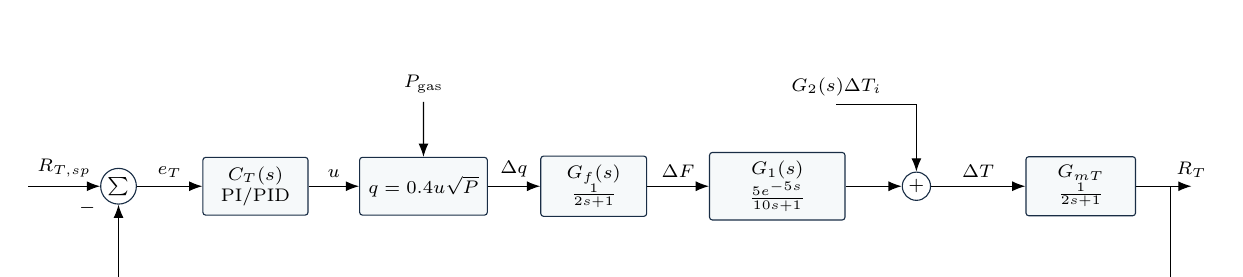
\begin{tikzpicture}[>=Latex,font=\scriptsize,x=1cm,y=1cm,scale=.94,transform shape,
block/.style={draw=ink,rounded corners=1pt,fill=accent!4,align=center,minimum height=.78cm},
node/.style={circle,draw=ink,inner sep=1pt,minimum size=.38cm}]
\node[node] (sum) at (1.3,0) {$\sum$};
\node[block,minimum width=1.42cm] (tc) at (3.15,0) {$C_T(s)$\\\scriptsize PI/PID};
\node[block,minimum width=1.68cm] (v) at (5.42,0) {$q=0.4u\sqrt{P}$};
\node[block,minimum width=1.43cm] (f) at (7.72,0) {$G_f(s)$\\$\frac{1}{2s+1}$};
\node[block,minimum width=1.83cm] (heat) at (10.20,0) {$G_1(s)$\\$\frac{5e^{-5s}}{10s+1}$};
\node[node] (add) at (12.08,0) {$+$};
\node[block,minimum width=1.48cm] (m) at (14.3,0) {$G_{mT}$\\ $\frac{1}{2s+1}$};
\draw[->] (.08,0) -- node[above]{$R_{T,sp}$}(sum);
\draw[->] (sum)--node[above]{$e_T$}(tc);
\draw[->] (tc)--node[above]{$u$}(v);
\draw[->] (v)--node[above]{$\dev q$}(f);
\draw[->] (f)--node[above]{$\dev F$}(heat);
\draw[->] (heat)--(add);
\draw[->] (add)--node[above]{$\dev T$}(m);
\draw[->] (m.east)--++(.75,0)node[above]{$R_T$};
\draw[->] (5.42,1.14)node[above]{$P_{\mathrm{gas}}$}--(v.north);
\draw[->] (11.0,1.1)node[above]{$G_2(s)\dev T_i$} -| (add.north);
\draw[->] (m.east)++(.47,0) |- (8.4,-1.36) -| (sum.south);
\node[anchor=east,fill=white,inner sep=1pt] at (1.03,-.30){$-$};
\end{tikzpicture}
\end{center}
图中为\textbf{偏差信号骨架}；$q-q_0$、$T_0$ 以及式\eqref{eq:meas}的量程归一化与偏置应在 Simulink 中补齐。单回路\textbf{只闭合温度反馈}，燃气流量可以用 Scope 观测，但不送回温控器形成副回路。

\subsection{串级控制：温度主回路 + 燃气流量副回路}
温控器 $TC$ 输出\textbf{流量设定值 $R_{F,sp}$}；流控器 $FC$ 比较 $R_{F,sp}$ 与 $R_F$，其输出才是阀门命令 $u$。两只调节器均以设定值减测量值为误差，并取正比例参数。
\begin{center}
\begin{tikzpicture}[>=Latex,font=\scriptsize,x=1cm,y=1cm,scale=.94,transform shape,
block/.style={draw=ink,rounded corners=1pt,fill=accent!4,align=center,minimum height=.8cm},
node/.style={circle,draw=ink,inner sep=1pt,minimum size=.38cm}]
\node[node] (st) at (1.0,0) {$\sum$};
\node[block,minimum width=1.20cm] (tc) at (2.55,0) {$TC$};
\node[node] (sf) at (4.27,0) {$\sum$};
\node[block,minimum width=1.20cm] (fc) at (5.82,0) {$FC$};
\node[block,minimum width=1.46cm] (val) at (7.87,0) {阀门\\ $q(u,P)$};
\node[block,minimum width=1.36cm] (flow) at (9.89,0) {$G_f(s)$};
\node[block,minimum width=1.32cm] (temp) at (12.02,0) {$G_1(s)$};
\node[node] (add) at (13.54,0) {$+$};
\node[block,minimum width=1.26cm] (tm) at (15.18,0) {$G_{mT}$};
\node[block,minimum width=1.25cm] (fm) at (9.89,-1.5) {$G_{mF}$};
\draw[->](0,0)node[above]{$R_{T,sp}$}--(st);
\draw[->](st)--(tc);
\draw[->](tc)--node[above]{$R_{F,sp}$}(sf);
\draw[->](sf)--(fc);
\draw[->](fc)--node[above]{$u$}(val);
\draw[->](val)--(flow);
\draw[->](flow)--node[above]{$\dev F$}(temp);
\draw[->](temp)--(add);
\draw[->](add)--node[above]{$T$}(tm);
\draw[->](tm.east)--++(.38,0)node[above]{$R_T$};
\draw[->](7.87,1)node[above]{$P_{\rm gas}$}--(val);
\draw[->](12.85,1)node[above]{$G_2(s)\dev T_i$}-|(add);
\draw[->](flow.south)--(fm.north);
\draw[->](fm.west)-|(sf.south);
\draw[->](tm.east)++(.3,0) |- (7.17,-2.37) -| (st.south);
\node[anchor=east,fill=white,inner sep=1pt] at (4.02,-.25){$-$};
\node[anchor=east,fill=white,inner sep=1pt] at (.73,-.25){$-$};
\end{tikzpicture}
\end{center}
流量变送器 $G_{mF}(s)=\frac{2.5}{0.2s+1}$；温度变送器按式\eqref{eq:meas}实现。$G_1$ 中含 $5\unit{min}$ 纯滞后。仿真时先把主回路置于手动、整定流量副回路，确认其快速稳定，再闭合主回路。

\section{（2）控制器整定与扰动比较}
\subsection{求线性化增益与给出参考整定值}
在 $(u_0,P_{\rm gas,0})=(60,0.25)$ 处一阶线性化式\eqref{eq:valve}：
\begin{align}
\dev q &\approx \frac{\partial q}{\partial u}\bigg|_0\dev u+\frac{\partial q}{\partial P}\bigg|_0\dev P
=\underbrace{0.4\sqrt{0.25}}_{0.2}\dev u
+\underbrace{\frac{0.4\times60}{2\sqrt{0.25}}}_{24}\dev P.\label{eq:linear}
\end{align}
以百分量计，阀门命令 $u\rightarrow R_F$ 的局部对象增益为 $K_{uF}=2.5\times0.2=0.5$；阀门命令 $u\rightarrow R_T$ 的局部对象增益为 $K_{uT}=0.5\times5\times0.2=0.5$。于是\textbf{单回路温度开环对象}为
\begin{equation}
G_{uR_T}(s)=\frac{0.5e^{-5s}}{(2s+1)^2(10s+1)},\qquad
G_{uR_F}(s)=\frac{0.5}{(2s+1)(0.2s+1)}.
\end{equation}
注意右式包含了\textbf{副回路流量变送器的 $0.2\unit{min}$ 动态}，不应漏掉。

\textbf{整定方案：}先按保守 IMC/$\lambda$ 思路给出初始范围，再通过闭环阶跃观察调整。下表给出本文独立等效仿真\textbf{确实采用}的参考参数（调节器输入、输出均为\textbf{\% span}，$t$ 用分钟）。下表 $T_d=0$ 属于 PID 的 PI 退化情形；题目没有指定必须保留非零微分项，也没有给唯一的 PID 参数。
\begin{center}
\small
\begin{tabular}{p{.32\linewidth}rrrrp{.17\linewidth}}
\toprule
回路 & $K_p$ & $T_i/\mathrm{min}$ & $T_d/\mathrm{min}$ & $K_i=K_p/T_i$ & 输出 \\
\midrule
单回路温控 $TC$ & $1.00$ & $10.0$ & $0$ & $0.100$ & 阀门 $u/\%$\\
串级流量副回路 $FC$ & $2.40$ & $2.0$ & $0$ & $1.200$ & 阀门 $u/\%$\\
串级温度主回路 $TC$ & $0.55$ & $10.0$ & $0$ & $0.055$ & $R_{F,sp}/\%$\\
\bottomrule
\end{tabular}
\end{center}
\begin{warnbox}
\textbf{Simulink PID Block 填参注意：}如果控制器采用\texttt{Parallel}参数形式，应填 $P=K_p$、$I=K_i=K_p/T_i$、$D=K_pT_d$，\textbf{不能把积分时间 $T_i=10$ 当作积分增益 $I=10$}。若使用\texttt{Ideal}形式才以 $K_p,T_i,T_d$ 为主。同时应设置工作点偏置：单回路 $u_0=60\%$，串级主回路 $R_{F,sp,0}=30\%$，副回路 $u_0=60\%$；或等效地设置积分器初值。
\end{warnbox}

如需非零微分项的完整 PID 对照试验，可在\textbf{上述 PI 稳定闭环之后}，对温度主回路试加小量带滤波的 $T_d$，逐项比较超调、峰值、抗噪声与阀门动作，\textbf{不能无仿真依据地把额外的非零微分参数写成唯一标准答案}。流量副环通常优先 PI。

\subsection{干扰设定与独立数值仿真}
题目要求比较 $P_{\rm gas}$ 与 $T_i$ 两种扰动，但\textbf{未固定阶跃幅值和发生时刻}。为了给出可复现的一组\textbf{演示参考}，本文自行设定：初始 $20\unit{min}$ 稳定，在 $t=20\unit{min}$ 时分别施加
\begin{align}
\text{试验 A：}&\quad P_{\rm gas}: 0.25\rightarrow0.16\unit{MPa},\quad T_i=120\unit{^\circ C};\\
\text{试验 B：}&\quad T_i:120\rightarrow140\unit{^\circ C},\quad P_{\rm gas}=0.25\unit{MPa}.
\end{align}
两个干扰分开测试，$T_{sp}=300\unit{^\circ C}$ 不变。参考曲线由\textbf{步长 $\dev t=0.02\unit{min}$ 的一阶动态递推与 $5\unit{min}$ 纯滞后队列}生成，数值设置、参数和基准完全相同。不是从题目附带的 Simulink 图中读取的测量结果。

\begin{center}
\begin{tikzpicture}
\begin{axis}[
width=.97\linewidth,height=6.1cm,
xmin=0,xmax=120,ymin=289,ymax=303,
xtick={0,20,40,60,80,100,120},
xlabel={时间 / min},ylabel={炉出口温度 / $^\circ$C},
legend style={at={(0.98,0.02)},anchor=south east,font=\footnotesize,draw=none,fill=white},
grid=both,major grid style={line!80},minor grid style={line!35},
tick label style={font=\footnotesize},label style={font=\small}]
\addplot[color=accent,very thick] coordinates {(0.0,300.000) (0.6,300.000) (1.2,300.000) (1.8,300.000) (2.4,300.000) (3.0,300.000) (3.6,300.000) (4.2,300.000) (4.8,300.000) (5.4,300.000) (6.0,300.000) (6.6,300.000) (7.2,300.000) (7.8,300.000) (8.4,300.000) (9.0,300.000) (9.6,300.000) (10.2,300.000) (10.8,300.000) (11.4,300.000) (12.0,300.000) (12.6,300.000) (13.2,300.000) (13.8,300.000) (14.4,300.000) (15.0,300.000) (15.6,300.000) (16.2,300.000) (16.8,300.000) (17.4,300.000) (18.0,300.000) (18.6,300.000) (19.2,300.000) (19.8,300.000) (20.4,300.000) (21.0,300.000) (21.6,300.000) (22.2,300.000) (22.8,300.000) (23.4,300.000) (24.0,300.000) (24.6,300.000) (25.2,299.990) (25.8,299.840) (26.4,299.556) (27.0,299.184) (27.6,298.756) (28.2,298.294) (28.8,297.817) (29.4,297.336) (30.0,296.860) (30.6,296.393) (31.2,295.942) (31.8,295.507) (32.4,295.091) (33.0,294.697) (33.6,294.325) (34.2,293.975) (34.8,293.650) (35.4,293.350) (36.0,293.074) (36.6,292.823) (37.2,292.596) (37.8,292.394) (38.4,292.216) (39.0,292.061) (39.6,291.929) (40.2,291.818) (40.8,291.729) (41.4,291.659) (42.0,291.609) (42.6,291.577) (43.2,291.563) (43.8,291.565) (44.4,291.582) (45.0,291.613) (45.6,291.658) (46.2,291.715) (46.8,291.784) (47.4,291.864) (48.0,291.953) (48.6,292.052) (49.2,292.158) (49.8,292.272) (50.4,292.393) (51.0,292.519) (51.6,292.651) (52.2,292.787) (52.8,292.927) (53.4,293.071) (54.0,293.217) (54.6,293.366) (55.2,293.516) (55.8,293.668) (56.4,293.821) (57.0,293.974) (57.6,294.128) (58.2,294.281) (58.8,294.434) (59.4,294.586) (60.0,294.737) (60.6,294.887) (61.2,295.036) (61.8,295.183) (62.4,295.328) (63.0,295.470) (63.6,295.611) (64.2,295.749) (64.8,295.885) (65.4,296.019) (66.0,296.150) (66.6,296.278) (67.2,296.403) (67.8,296.526) (68.4,296.646) (69.0,296.763) (69.6,296.877) (70.2,296.988) (70.8,297.097) (71.4,297.202) (72.0,297.305) (72.6,297.404) (73.2,297.501) (73.8,297.595) (74.4,297.687) (75.0,297.775) (75.6,297.861) (76.2,297.944) (76.8,298.025) (77.4,298.103) (78.0,298.178) (78.6,298.251) (79.2,298.321) (79.8,298.389) (80.4,298.455) (81.0,298.518) (81.6,298.579) (82.2,298.638) (82.8,298.695) (83.4,298.750) (84.0,298.803) (84.6,298.854) (85.2,298.903) (85.8,298.950) (86.4,298.995) (87.0,299.039) (87.6,299.081) (88.2,299.121) (88.8,299.159) (89.4,299.197) (90.0,299.232) (90.6,299.266) (91.2,299.299) (91.8,299.331) (92.4,299.361) (93.0,299.390) (93.6,299.418) (94.2,299.444) (94.8,299.470) (95.4,299.494) (96.0,299.518) (96.6,299.540) (97.2,299.562) (97.8,299.582) (98.4,299.602) (99.0,299.621) (99.6,299.639) (100.2,299.656) (100.8,299.672) (101.4,299.688) (102.0,299.703) (102.6,299.717) (103.2,299.731) (103.8,299.744) (104.4,299.756) (105.0,299.768) (105.6,299.779) (106.2,299.790) (106.8,299.801) (107.4,299.810) (108.0,299.820) (108.6,299.829) (109.2,299.837) (109.8,299.845) (110.4,299.853) (111.0,299.861) (111.6,299.868) (112.2,299.874) (112.8,299.881) (113.4,299.887) (114.0,299.892) (114.6,299.898) (115.2,299.903) (115.8,299.908) (116.4,299.913) (117.0,299.917) (117.6,299.922) (118.2,299.926) (118.8,299.930) (119.4,299.933) (120.0,299.937)};\addlegendentry{单回路}
\addplot[color=copper,very thick,dashed] coordinates {(0.0,300.000) (0.6,300.000) (1.2,300.000) (1.8,300.000) (2.4,300.000) (3.0,300.000) (3.6,300.000) (4.2,300.000) (4.8,300.000) (5.4,300.000) (6.0,300.000) (6.6,300.000) (7.2,300.000) (7.8,300.000) (8.4,300.000) (9.0,300.000) (9.6,300.000) (10.2,300.000) (10.8,300.000) (11.4,300.000) (12.0,300.000) (12.6,300.000) (13.2,300.000) (13.8,300.000) (14.4,300.000) (15.0,300.000) (15.6,300.000) (16.2,300.000) (16.8,300.000) (17.4,300.000) (18.0,300.000) (18.6,300.000) (19.2,300.000) (19.8,300.000) (20.4,300.000) (21.0,300.000) (21.6,300.000) (22.2,300.000) (22.8,300.000) (23.4,300.000) (24.0,300.000) (24.6,300.000) (25.2,299.990) (25.8,299.850) (26.4,299.620) (27.0,299.367) (27.6,299.129) (28.2,298.925) (28.8,298.763) (29.4,298.641) (30.0,298.558) (30.6,298.508) (31.2,298.486) (31.8,298.487) (32.4,298.506) (33.0,298.542) (33.6,298.590) (34.2,298.649) (34.8,298.717) (35.4,298.792) (36.0,298.873) (36.6,298.959) (37.2,299.048) (37.8,299.139) (38.4,299.232) (39.0,299.325) (39.6,299.417) (40.2,299.509) (40.8,299.598) (41.4,299.686) (42.0,299.771) (42.6,299.852) (43.2,299.931) (43.8,300.005) (44.4,300.076) (45.0,300.143) (45.6,300.206) (46.2,300.264) (46.8,300.319) (47.4,300.369) (48.0,300.415) (48.6,300.457) (49.2,300.495) (49.8,300.529) (50.4,300.560) (51.0,300.586) (51.6,300.609) (52.2,300.629) (52.8,300.645) (53.4,300.658) (54.0,300.668) (54.6,300.676) (55.2,300.680) (55.8,300.683) (56.4,300.682) (57.0,300.680) (57.6,300.676) (58.2,300.670) (58.8,300.662) (59.4,300.653) (60.0,300.642) (60.6,300.630) (61.2,300.617) (61.8,300.603) (62.4,300.589) (63.0,300.573) (63.6,300.557) (64.2,300.540) (64.8,300.523) (65.4,300.505) (66.0,300.488) (66.6,300.470) (67.2,300.452) (67.8,300.434) (68.4,300.416) (69.0,300.398) (69.6,300.380) (70.2,300.363) (70.8,300.346) (71.4,300.329) (72.0,300.312) (72.6,300.296) (73.2,300.280) (73.8,300.265) (74.4,300.250) (75.0,300.235) (75.6,300.221) (76.2,300.207) (76.8,300.194) (77.4,300.182) (78.0,300.170) (78.6,300.158) (79.2,300.147) (79.8,300.136) (80.4,300.126) (81.0,300.116) (81.6,300.107) (82.2,300.098) (82.8,300.090) (83.4,300.082) (84.0,300.075) (84.6,300.068) (85.2,300.061) (85.8,300.055) (86.4,300.049) (87.0,300.044) (87.6,300.039) (88.2,300.034) (88.8,300.030) (89.4,300.026) (90.0,300.022) (90.6,300.019) (91.2,300.015) (91.8,300.012) (92.4,300.010) (93.0,300.007) (93.6,300.005) (94.2,300.003) (94.8,300.001) (95.4,300.000) (96.0,299.998) (96.6,299.997) (97.2,299.996) (97.8,299.995) (98.4,299.994) (99.0,299.993) (99.6,299.993) (100.2,299.992) (100.8,299.992) (101.4,299.991) (102.0,299.991) (102.6,299.991) (103.2,299.991) (103.8,299.991) (104.4,299.991) (105.0,299.991) (105.6,299.991) (106.2,299.991) (106.8,299.991) (107.4,299.991) (108.0,299.992) (108.6,299.992) (109.2,299.992) (109.8,299.992) (110.4,299.993) (111.0,299.993) (111.6,299.993) (112.2,299.994) (112.8,299.994) (113.4,299.994) (114.0,299.995) (114.6,299.995) (115.2,299.995) (115.8,299.996) (116.4,299.996) (117.0,299.996) (117.6,299.996) (118.2,299.997) (118.8,299.997) (119.4,299.997) (120.0,299.997)};\addlegendentry{串级}
\addplot[color=gray,dotted] coordinates {(0,300)(120,300)};
\addplot[color=muted,dotted] coordinates {(20,289)(20,303)};
\end{axis}
\end{tikzpicture}
\par\footnotesize\color{muted} 图 1 · 燃气压力下降（$0.25\rightarrow0.16\unit{MPa}$）时的温度响应；虚线表示干扰时刻。\par
\end{center}
\begin{center}
\begin{tikzpicture}
\begin{axis}[
width=.97\linewidth,height=6.1cm,
xmin=0,xmax=120,ymin=297,ymax=322,
xtick={0,20,40,60,80,100,120},
xlabel={时间 / min},ylabel={炉出口温度 / $^\circ$C},
legend style={at={(0.98,0.98)},anchor=north east,font=\footnotesize,draw=none,fill=white},
grid=both,major grid style={line!80},minor grid style={line!35},
tick label style={font=\footnotesize},label style={font=\small}]
\addplot[color=accent,very thick] coordinates {(0.0,300.000) (0.6,300.000) (1.2,300.000) (1.8,300.000) (2.4,300.000) (3.0,300.000) (3.6,300.000) (4.2,300.000) (4.8,300.000) (5.4,300.000) (6.0,300.000) (6.6,300.000) (7.2,300.000) (7.8,300.000) (8.4,300.000) (9.0,300.000) (9.6,300.000) (10.2,300.000) (10.8,300.000) (11.4,300.000) (12.0,300.000) (12.6,300.000) (13.2,300.000) (13.8,300.000) (14.4,300.000) (15.0,300.000) (15.6,300.000) (16.2,300.000) (16.8,300.000) (17.4,300.000) (18.0,300.000) (18.6,300.000) (19.2,300.000) (19.8,300.000) (20.4,306.594) (21.0,312.642) (21.6,315.962) (22.2,317.784) (22.8,318.784) (23.4,319.333) (24.0,319.634) (24.6,319.799) (25.2,319.890) (25.8,319.937) (26.4,319.945) (27.0,319.907) (27.6,319.815) (28.2,319.664) (28.8,319.452) (29.4,319.184) (30.0,318.862) (30.6,318.492) (31.2,318.082) (31.8,317.637) (32.4,317.161) (33.0,316.662) (33.6,316.143) (34.2,315.608) (34.8,315.062) (35.4,314.508) (36.0,313.948) (36.6,313.386) (37.2,312.824) (37.8,312.265) (38.4,311.710) (39.0,311.162) (39.6,310.622) (40.2,310.091) (40.8,309.570) (41.4,309.062) (42.0,308.566) (42.6,308.083) (43.2,307.615) (43.8,307.162) (44.4,306.723) (45.0,306.300) (45.6,305.893) (46.2,305.501) (46.8,305.125) (47.4,304.766) (48.0,304.421) (48.6,304.093) (49.2,303.780) (49.8,303.482) (50.4,303.199) (51.0,302.931) (51.6,302.677) (52.2,302.437) (52.8,302.210) (53.4,301.997) (54.0,301.796) (54.6,301.608) (55.2,301.431) (55.8,301.266) (56.4,301.112) (57.0,300.969) (57.6,300.836) (58.2,300.712) (58.8,300.597) (59.4,300.492) (60.0,300.394) (60.6,300.305) (61.2,300.223) (61.8,300.148) (62.4,300.080) (63.0,300.018) (63.6,299.963) (64.2,299.913) (64.8,299.868) (65.4,299.828) (66.0,299.792) (66.6,299.762) (67.2,299.735) (67.8,299.711) (68.4,299.692) (69.0,299.675) (69.6,299.661) (70.2,299.650) (70.8,299.642) (71.4,299.636) (72.0,299.632) (72.6,299.630) (73.2,299.629) (73.8,299.631) (74.4,299.633) (75.0,299.637) (75.6,299.642) (76.2,299.648) (76.8,299.655) (77.4,299.662) (78.0,299.670) (78.6,299.679) (79.2,299.688) (79.8,299.698) (80.4,299.708) (81.0,299.718) (81.6,299.728) (82.2,299.738) (82.8,299.749) (83.4,299.759) (84.0,299.770) (84.6,299.780) (85.2,299.790) (85.8,299.800) (86.4,299.810) (87.0,299.820) (87.6,299.829) (88.2,299.838) (88.8,299.847) (89.4,299.856) (90.0,299.865) (90.6,299.873) (91.2,299.881) (91.8,299.888) (92.4,299.896) (93.0,299.903) (93.6,299.910) (94.2,299.916) (94.8,299.922) (95.4,299.928) (96.0,299.934) (96.6,299.939) (97.2,299.944) (97.8,299.949) (98.4,299.953) (99.0,299.958) (99.6,299.962) (100.2,299.965) (100.8,299.969) (101.4,299.972) (102.0,299.975) (102.6,299.978) (103.2,299.981) (103.8,299.984) (104.4,299.986) (105.0,299.988) (105.6,299.990) (106.2,299.992) (106.8,299.994) (107.4,299.995) (108.0,299.997) (108.6,299.998) (109.2,299.999) (109.8,300.000) (110.4,300.001) (111.0,300.002) (111.6,300.003) (112.2,300.003) (112.8,300.004) (113.4,300.005) (114.0,300.005) (114.6,300.005) (115.2,300.006) (115.8,300.006) (116.4,300.006) (117.0,300.006) (117.6,300.007) (118.2,300.007) (118.8,300.007) (119.4,300.007) (120.0,300.007)};\addlegendentry{单回路}
\addplot[color=copper,very thick,dashed] coordinates {(0.0,300.000) (0.6,300.000) (1.2,300.000) (1.8,300.000) (2.4,300.000) (3.0,300.000) (3.6,300.000) (4.2,300.000) (4.8,300.000) (5.4,300.000) (6.0,300.000) (6.6,300.000) (7.2,300.000) (7.8,300.000) (8.4,300.000) (9.0,300.000) (9.6,300.000) (10.2,300.000) (10.8,300.000) (11.4,300.000) (12.0,300.000) (12.6,300.000) (13.2,300.000) (13.8,300.000) (14.4,300.000) (15.0,300.000) (15.6,300.000) (16.2,300.000) (16.8,300.000) (17.4,300.000) (18.0,300.000) (18.6,300.000) (19.2,300.000) (19.8,300.000) (20.4,306.594) (21.0,312.642) (21.6,315.962) (22.2,317.784) (22.8,318.784) (23.4,319.333) (24.0,319.634) (24.6,319.799) (25.2,319.890) (25.8,319.936) (26.4,319.937) (27.0,319.880) (27.6,319.752) (28.2,319.550) (28.8,319.274) (29.4,318.930) (30.0,318.526) (30.6,318.070) (31.2,317.571) (31.8,317.038) (32.4,316.476) (33.0,315.892) (33.6,315.292) (34.2,314.679) (34.8,314.059) (35.4,313.435) (36.0,312.810) (36.6,312.188) (37.2,311.571) (37.8,310.962) (38.4,310.362) (39.0,309.774) (39.6,309.199) (40.2,308.640) (40.8,308.096) (41.4,307.569) (42.0,307.060) (42.6,306.569) (43.2,306.097) (43.8,305.645) (44.4,305.212) (45.0,304.798) (45.6,304.404) (46.2,304.029) (46.8,303.674) (47.4,303.337) (48.0,303.020) (48.6,302.720) (49.2,302.438) (49.8,302.174) (50.4,301.926) (51.0,301.695) (51.6,301.479) (52.2,301.278) (52.8,301.092) (53.4,300.920) (54.0,300.762) (54.6,300.616) (55.2,300.482) (55.8,300.359) (56.4,300.248) (57.0,300.147) (57.6,300.056) (58.2,299.973) (58.8,299.900) (59.4,299.834) (60.0,299.777) (60.6,299.726) (61.2,299.682) (61.8,299.644) (62.4,299.611) (63.0,299.584) (63.6,299.562) (64.2,299.544) (64.8,299.530) (65.4,299.520) (66.0,299.513) (66.6,299.509) (67.2,299.508) (67.8,299.510) (68.4,299.514) (69.0,299.519) (69.6,299.527) (70.2,299.536) (70.8,299.546) (71.4,299.557) (72.0,299.570) (72.6,299.583) (73.2,299.597) (73.8,299.611) (74.4,299.626) (75.0,299.641) (75.6,299.656) (76.2,299.672) (76.8,299.687) (77.4,299.702) (78.0,299.717) (78.6,299.732) (79.2,299.747) (79.8,299.761) (80.4,299.775) (81.0,299.789) (81.6,299.802) (82.2,299.815) (82.8,299.828) (83.4,299.840) (84.0,299.851) (84.6,299.862) (85.2,299.873) (85.8,299.883) (86.4,299.892) (87.0,299.902) (87.6,299.910) (88.2,299.918) (88.8,299.926) (89.4,299.934) (90.0,299.940) (90.6,299.947) (91.2,299.953) (91.8,299.959) (92.4,299.964) (93.0,299.969) (93.6,299.973) (94.2,299.977) (94.8,299.981) (95.4,299.985) (96.0,299.988) (96.6,299.991) (97.2,299.994) (97.8,299.996) (98.4,299.998) (99.0,300.000) (99.6,300.002) (100.2,300.004) (100.8,300.005) (101.4,300.007) (102.0,300.008) (102.6,300.009) (103.2,300.009) (103.8,300.010) (104.4,300.011) (105.0,300.011) (105.6,300.011) (106.2,300.012) (106.8,300.012) (107.4,300.012) (108.0,300.012) (108.6,300.012) (109.2,300.012) (109.8,300.012) (110.4,300.011) (111.0,300.011) (111.6,300.011) (112.2,300.011) (112.8,300.010) (113.4,300.010) (114.0,300.010) (114.6,300.009) (115.2,300.009) (115.8,300.009) (116.4,300.008) (117.0,300.008) (117.6,300.008) (118.2,300.007) (118.8,300.007) (119.4,300.006) (120.0,300.006)};\addlegendentry{串级}
\addplot[color=gray,dotted] coordinates {(0,300)(120,300)};
\addplot[color=muted,dotted] coordinates {(20,297)(20,322)};
\end{axis}
\end{tikzpicture}
\par\footnotesize\color{muted} 图 2 · 入口温度升高（$120\rightarrow140\unit{^\circ C}$）时的温度响应。\par
\end{center}

\begin{center}
\small
\begin{tabular}{p{.13\linewidth}p{.14\linewidth} >{\centering\arraybackslash}p{.22\linewidth} >{\centering\arraybackslash}p{.17\linewidth} >{\centering\arraybackslash}p{.18\linewidth}}
\toprule
干扰 & 控制方案 & 峰值绝对偏差 / $^\circ$C & IAE / ($^\circ$C\,min) & 回到 $\pm1^\circ$C / min \\
\midrule
$P_{\rm gas}\downarrow$ & 单回路 & 8.44 & 299.90 & 66.48\\
& 串级 & 1.52 & 33.38 & 16.88\\
$T_i\uparrow$ & 单回路 & 19.95 & 416.09 & 36.88\\
& 串级 & 19.94 & 383.03 & 33.12\\
\bottomrule
\end{tabular}
\par\footnotesize\color{muted} 表 1 · 仅为上述参数与扰动条件下的独立数值仿真参考，不是题目给出的标准实测值。\par
\end{center}

\task{结论与作用机理}
\begin{enumerate}
\item \textbf{燃气压力扰动：}压力下降使 $q=K_{\rm gas}u\sqrt{P}$ 立即减小；副回路的 $FT$ 能够在温度出现明显变化\emph{之前}检测流量下降，快速增大 $u$，因而显著抑制温度波动。单回路只能等待受 $G_1$ 滞后与延迟影响的温度反馈，动作较慢。
\item \textbf{入口温度扰动：}$T_i$ 直接经 $G_2(s)$ 进入温度通道，不首先造成燃气流量测量变化，因此流量副回路\textbf{无法提前感知}；改善主要依靠温度主回路。两种控制方案的\textbf{初始温度峰值可能基本一样}，串级不保证对该类扰动总是显著优越。
\item \textbf{稳态检查：}在无测量偏差且能满足执行器约束时，积分作用应使 $T\to300\unit{^\circ C}$。试验 A 压力由 $0.25$ 降为 $0.16\unit{MPa}$，恢复 $F=12$ 的稳态阀命令应为 $u=12/(0.4\sqrt{0.16})=75\%$；试验 B 入口温度增 $20^\circ$C，若热通道静态增益 $5$ 不变，稳态应减少 $\dev F=-20/5=-4\unit{T/hr}$，即 $F=8\unit{T/hr}$、$u=40\%$。数值参考结果满足该物理一致性检查。
\end{enumerate}

\section{（3）主回路抗积分饱和（Anti-windup）}
串级系统主回路 $TC$ 的输出是\textbf{流量给定值}，而非直接的阀命令。首先把主回路输出限制在可实现的流量设定范围内，推荐\textbf{反算跟踪法}（back-calculation）：
\begin{align}
v_T(t)&=R_{F,sp,0}+K_{pT}e_T(t)+I_T(t)+D_T(t),\\
R_{F,sp}(t)&=\operatorname{sat}\big(v_T(t);R_{F,\min},R_{F,\max}\big),\\
\dot I_T(t)&=K_{iT}e_T(t)+\frac{R_{F,sp}(t)-v_T(t)}{T_{aw}},\label{eq:aw}
\end{align}
其中 $e_T=R_{T,sp}-R_T$，可先按变送器范围取 $R_{F,\min}=0\%$、$R_{F,\max}=100\%$；$T_{aw}>0$ 为跟踪时间常数，\textbf{例如初步取 $3\unit{min}$ 后再通过饱和恢复实验整定}。若主回路仍采用 PI，则 $D_T=0$。

\begin{center}
\begin{tikzpicture}[>=Latex,thick,font=\small,
block/.style={draw=ink,fill=accent!4,rounded corners=1pt,minimum width=2.1cm,minimum height=.8cm,align=center},
add/.style={circle,draw=ink,minimum size=.6cm,inner sep=0pt}]
\node[add] (join) at (2.0,0) {$\sum$};
\node[block] (sat) at (6.0,0) {$\operatorname{sat}(v_T)$};
\node[block] (track) at (6.0,-1.7) {$(R_{F,sp}-v_T)/T_{aw}$};
\node[block] (integ) at (2.0,-1.7) {积分器 $I_T$};
\draw[->](0,0)node[above]{$R_{F,sp,0}+K_pe_T+D_T$}--(join);
\draw[->](join)--node[above]{$v_T$}(sat);
\draw[->](sat.east)--++(1.4,0) node[above]{$R_{F,sp}$};
\draw[->](sat.east)++(.85,0) |- (track.east);
\draw[->](join.east)++(.9,0) |- (3.85,-2.4) -| (track.south);
\draw[->](track)--(integ);
\draw[->](integ.north)--(join.south);
\node[font=\scriptsize,align=center] at (1.0,-2.5) {$K_i e_T$ 同时进入积分器};
\end{tikzpicture}
\par\footnotesize\color{muted} 图 3 · 主控制器的饱和输出反馈到积分通道，用于停止无约束积分增长（结构示意）。\par
\end{center}

\textbf{工作过程：}当要求的流量给定超过上限时，$R_{F,sp}<v_T$，则式\eqref{eq:aw}中跟踪项为负，把积分状态往回拉；恢复到可控范围后，积分快速回归，不会因先前积累过大产生持续超调。下限饱和同理。还应对\textbf{副回路阀门命令 $u\in[0,100]\%$} 设置饱和和防积分饱和，避免副回路本身 windup。

\begin{warnbox}
\textbf{串级系统的额外风险：}即便 $R_{F,sp}$ 位于 $0\sim100\%$，副环阀门可能已打满仍达不到目标流量（例如 $P_{\rm gas}=0.25\unit{MPa}$ 时 $u\le100\%$ 给出的稳态 $F\le20\unit{T/hr}$，仅占 FT 量程 $50\%$）。因此应结合\textbf{副环执行器饱和信息和实际测量流量}进行主回路外部复位跟踪（external-reset feedback），或动态限制主回路可实现的流量给定，而不只按变送器量程限制。
\end{warnbox}

\section{Simulink 复现实验与提交检查}
\task{步骤 A：建模与零扰动自检}
\begin{enumerate}
\item 用 \texttt{Constant} 初始化 $P_{\rm gas}=0.25$、$u_0=60$、$T_i=120$、$F_0=12$、$T_0=300$，各一阶传函的初始状态设置为其绝对或偏差模型对应的稳态值；确认零扰动时 $F_{\rm gas}=12$、$T=300$、$R_F=30\%$、$R_T=50\%$。
\item 添加 \texttt{Transport Delay}，延迟 $5\unit{min}$，延迟环节的初始输出在偏差模型中应为 $0$；区分模型中的 $T_{m1}=2$ 与 $T_{m2}=0.2$。
\item 实现并分别保留单回路和串级两种控制结构：两者必须\textbf{共用完全一致的被控对象参数与扰动工况}，否则比较不公平。
\end{enumerate}
\task{步骤 B：整定与比较}
\begin{enumerate}
\item 单回路先用表中参考 PI 参数运行设定值小阶跃、再测试压力与入口温度扰动；必要时降低比例增益、延长积分时间。
\item 串级先闭合 $FC$，先证实\textbf{流量阶跃响应明显快于温度回路}，然后闭合 $TC$；逐次保存调参过程中的关键曲线。
\item 建议 Scope / Data Inspector 至少采集 $P_{\rm gas},T_i,F_{\rm gas},F_m,T,T_m,R_{F,sp},u$；计算温度峰值偏差、积分绝对误差 $\mathrm{IAE}=\int|T(t)-T_{sp}|dt$ 和大致恢复时间。
\item 额外测试阀门 $0/100\%$ 或流量给定限幅，比较\textbf{有/无 anti-windup} 两种工况下的积分状态、解除饱和后的恢复时间及是否超调。
\end{enumerate}
\task{步骤 C：正式报告应放哪些图和表}
\begin{itemize}
\item \textbf{模型结构图：}单回路框图、串级框图、主回路防积分饱和内部结构（最好直接用自己的 Simulink 截图）。
\item \textbf{控制参数表：}$P$、$I$、$D$ 或 $K_p$、$T_i$、$T_d$，附控制器单位、输出范围和初始偏置。
\item \textbf{扰动响应：}同一张图叠加单回路 / 串级出口温度；另给流量和阀门命令以解释“为什么”改善，而不只是写“串级更好”。
\item \textbf{抗积分饱和：}给出主回路限幅、反算跟踪通路以及对比图；清楚说明只是避免积分累积，\textbf{不能突破阀门真实流量能力}。
\end{itemize}
\subsection*{Simulink 模块参数速查卡}
\begin{center}
\small
\begin{tabular}{>{\raggedright\arraybackslash}p{.33\linewidth}>{\raggedright\arraybackslash}p{.57\linewidth}}
\toprule
模块位置 & 填写建议（时间单位均为 min）\\
\midrule
$G_f$：燃气流量动态 & \texttt{Transfer Fcn}: Num=$[1]$, Den=$[2,1]$；输入 $q-12$，输出加 $12$\\
$G_1$：炉体升温 & \texttt{Transfer Fcn}: Num=$[5]$, Den=$[10,1]$；\texttt{Transport Delay}=5\\
$G_2$：入口温度 & \texttt{Transfer Fcn}: Num=$[1]$, Den=$[1,1]$；输入 $T_i-120$\\
$G_{mT}$：温度测量 & \texttt{Transfer Fcn}: Num=$[1]$, Den=$[2,1]$；随后减 200、乘 0.5\\
$G_{mF}$：流量测量 & \texttt{Transfer Fcn}: Num=$[1]$, Den=$[0.2,1]$；随后乘 2.5\\
操纵阀门 & \texttt{Saturation}: lower=0, upper=100；$u_0=60$\\
串级主控制器 & PI $P=0.55, I=0.055$，输出基准 $30\%$\\
串级副控制器 & PI $P=2.40, I=1.20$，输出基准 $60\%$\\
单回路温控器 & PI $P=1.00, I=0.10$，输出基准 $60\%$\\
\bottomrule
\end{tabular}
\end{center}
\noindent\textbf{注意：}含绝对流量、温度的传感器块应合理初始化；在\emph{纯偏差}信号上使用的传递函数初态则为零。若实际使用 \texttt{PID Controller} 模块并启用内置输出限幅或跟踪端口，应检查其 anti-windup 设置，避免外部与内部限幅/积分器叠加。

\vspace{1mm}
\begin{notebox}
\textbf{可以直接用于答题的总结：}燃气压力扰动位于\textbf{副回路以内}，流量副环提前纠偏，串级优势通常明显；入口温度扰动在\textbf{副回路以外}，只能经温度主环纠偏，串级优势较小或不稳定。主回路采用限幅 + 反算跟踪，并在副阀饱和时引入实际流量外部复位跟踪，可避免流量给定不可达导致的积分饱和。
\end{notebox}
\vspace{4mm}
\noindent\rule{\linewidth}{.3pt}
\noindent{\small\color{muted}\textbf{参考资料说明：}原题与工作点、动态参数来自《作业4(4).pptx》四页课件。文中的偏差域一致性处理、控制器试整定值、扰动幅值、独立数值仿真曲线和抗饱和扩展均为本参考解答的明确建模/实验选择，不属于教师给出的唯一参数或官方仿真结果。}
\end{document}